% Options for packages loaded elsewhere
\PassOptionsToPackage{unicode}{hyperref}
\PassOptionsToPackage{hyphens}{url}
\PassOptionsToPackage{dvipsnames,svgnames,x11names}{xcolor}
%
\documentclass[
  letterpaper,
  DIV=11,
  numbers=noendperiod]{scrartcl}

\usepackage{amsmath,amssymb}
\usepackage{iftex}
\ifPDFTeX
  \usepackage[T1]{fontenc}
  \usepackage[utf8]{inputenc}
  \usepackage{textcomp} % provide euro and other symbols
\else % if luatex or xetex
  \usepackage{unicode-math}
  \defaultfontfeatures{Scale=MatchLowercase}
  \defaultfontfeatures[\rmfamily]{Ligatures=TeX,Scale=1}
\fi
\usepackage{lmodern}
\ifPDFTeX\else  
    % xetex/luatex font selection
\fi
% Use upquote if available, for straight quotes in verbatim environments
\IfFileExists{upquote.sty}{\usepackage{upquote}}{}
\IfFileExists{microtype.sty}{% use microtype if available
  \usepackage[]{microtype}
  \UseMicrotypeSet[protrusion]{basicmath} % disable protrusion for tt fonts
}{}
\makeatletter
\@ifundefined{KOMAClassName}{% if non-KOMA class
  \IfFileExists{parskip.sty}{%
    \usepackage{parskip}
  }{% else
    \setlength{\parindent}{0pt}
    \setlength{\parskip}{6pt plus 2pt minus 1pt}}
}{% if KOMA class
  \KOMAoptions{parskip=half}}
\makeatother
\usepackage{xcolor}
\setlength{\emergencystretch}{3em} % prevent overfull lines
\setcounter{secnumdepth}{-\maxdimen} % remove section numbering
% Make \paragraph and \subparagraph free-standing
\makeatletter
\ifx\paragraph\undefined\else
  \let\oldparagraph\paragraph
  \renewcommand{\paragraph}{
    \@ifstar
      \xxxParagraphStar
      \xxxParagraphNoStar
  }
  \newcommand{\xxxParagraphStar}[1]{\oldparagraph*{#1}\mbox{}}
  \newcommand{\xxxParagraphNoStar}[1]{\oldparagraph{#1}\mbox{}}
\fi
\ifx\subparagraph\undefined\else
  \let\oldsubparagraph\subparagraph
  \renewcommand{\subparagraph}{
    \@ifstar
      \xxxSubParagraphStar
      \xxxSubParagraphNoStar
  }
  \newcommand{\xxxSubParagraphStar}[1]{\oldsubparagraph*{#1}\mbox{}}
  \newcommand{\xxxSubParagraphNoStar}[1]{\oldsubparagraph{#1}\mbox{}}
\fi
\makeatother


\providecommand{\tightlist}{%
  \setlength{\itemsep}{0pt}\setlength{\parskip}{0pt}}\usepackage{longtable,booktabs,array}
\usepackage{calc} % for calculating minipage widths
% Correct order of tables after \paragraph or \subparagraph
\usepackage{etoolbox}
\makeatletter
\patchcmd\longtable{\par}{\if@noskipsec\mbox{}\fi\par}{}{}
\makeatother
% Allow footnotes in longtable head/foot
\IfFileExists{footnotehyper.sty}{\usepackage{footnotehyper}}{\usepackage{footnote}}
\makesavenoteenv{longtable}
\usepackage{graphicx}
\makeatletter
\def\maxwidth{\ifdim\Gin@nat@width>\linewidth\linewidth\else\Gin@nat@width\fi}
\def\maxheight{\ifdim\Gin@nat@height>\textheight\textheight\else\Gin@nat@height\fi}
\makeatother
% Scale images if necessary, so that they will not overflow the page
% margins by default, and it is still possible to overwrite the defaults
% using explicit options in \includegraphics[width, height, ...]{}
\setkeys{Gin}{width=\maxwidth,height=\maxheight,keepaspectratio}
% Set default figure placement to htbp
\makeatletter
\def\fps@figure{htbp}
\makeatother
% definitions for citeproc citations
\NewDocumentCommand\citeproctext{}{}
\NewDocumentCommand\citeproc{mm}{%
  \begingroup\def\citeproctext{#2}\cite{#1}\endgroup}
\makeatletter
 % allow citations to break across lines
 \let\@cite@ofmt\@firstofone
 % avoid brackets around text for \cite:
 \def\@biblabel#1{}
 \def\@cite#1#2{{#1\if@tempswa , #2\fi}}
\makeatother
\newlength{\cslhangindent}
\setlength{\cslhangindent}{1.5em}
\newlength{\csllabelwidth}
\setlength{\csllabelwidth}{3em}
\newenvironment{CSLReferences}[2] % #1 hanging-indent, #2 entry-spacing
 {\begin{list}{}{%
  \setlength{\itemindent}{0pt}
  \setlength{\leftmargin}{0pt}
  \setlength{\parsep}{0pt}
  % turn on hanging indent if param 1 is 1
  \ifodd #1
   \setlength{\leftmargin}{\cslhangindent}
   \setlength{\itemindent}{-1\cslhangindent}
  \fi
  % set entry spacing
  \setlength{\itemsep}{#2\baselineskip}}}
 {\end{list}}
\usepackage{calc}
\newcommand{\CSLBlock}[1]{\hfill\break\parbox[t]{\linewidth}{\strut\ignorespaces#1\strut}}
\newcommand{\CSLLeftMargin}[1]{\parbox[t]{\csllabelwidth}{\strut#1\strut}}
\newcommand{\CSLRightInline}[1]{\parbox[t]{\linewidth - \csllabelwidth}{\strut#1\strut}}
\newcommand{\CSLIndent}[1]{\hspace{\cslhangindent}#1}

\usepackage{fontspec}
\usepackage{multirow}
\usepackage{multicol}
\usepackage{colortbl}
\usepackage{hhline}
\newlength\Oldarrayrulewidth
\newlength\Oldtabcolsep
\usepackage{longtable}
\usepackage{array}
\usepackage{hyperref}
\usepackage{float}
\usepackage{wrapfig}
\KOMAoption{captions}{tableheading}
\makeatletter
\@ifpackageloaded{caption}{}{\usepackage{caption}}
\AtBeginDocument{%
\ifdefined\contentsname
  \renewcommand*\contentsname{Table of contents}
\else
  \newcommand\contentsname{Table of contents}
\fi
\ifdefined\listfigurename
  \renewcommand*\listfigurename{List of Figures}
\else
  \newcommand\listfigurename{List of Figures}
\fi
\ifdefined\listtablename
  \renewcommand*\listtablename{List of Tables}
\else
  \newcommand\listtablename{List of Tables}
\fi
\ifdefined\figurename
  \renewcommand*\figurename{Figure}
\else
  \newcommand\figurename{Figure}
\fi
\ifdefined\tablename
  \renewcommand*\tablename{Table}
\else
  \newcommand\tablename{Table}
\fi
}
\@ifpackageloaded{float}{}{\usepackage{float}}
\floatstyle{ruled}
\@ifundefined{c@chapter}{\newfloat{codelisting}{h}{lop}}{\newfloat{codelisting}{h}{lop}[chapter]}
\floatname{codelisting}{Listing}
\newcommand*\listoflistings{\listof{codelisting}{List of Listings}}
\makeatother
\makeatletter
\makeatother
\makeatletter
\@ifpackageloaded{caption}{}{\usepackage{caption}}
\@ifpackageloaded{subcaption}{}{\usepackage{subcaption}}
\makeatother

\ifLuaTeX
  \usepackage{selnolig}  % disable illegal ligatures
\fi
\usepackage{bookmark}

\IfFileExists{xurl.sty}{\usepackage{xurl}}{} % add URL line breaks if available
\urlstyle{same} % disable monospaced font for URLs
\hypersetup{
  pdftitle={Age- and sex-standardised incidence of diabetes mellitus in Peru from 2016 to 2023},
  pdfauthor={Carlos J. Toro-Huamanchumo; Omar Silverman-Retana; Juan Pablo Perez Bedolla; Daniel R. Witte; Ralph Brinks; Thaddäus Tönnies},
  colorlinks=true,
  linkcolor={blue},
  filecolor={Maroon},
  citecolor={Blue},
  urlcolor={Blue},
  pdfcreator={LaTeX via pandoc}}


\title{Age- and sex-standardised incidence of diabetes mellitus in Peru
from 2016 to 2023}
\author{Carlos J. Toro-Huamanchumo \and Omar Silverman-Retana \and Juan
Pablo Perez Bedolla \and Daniel R. Witte \and Ralph Brinks \and Thaddäus
Tönnies}
\date{}

\begin{document}
\maketitle


\newpage{}

\section{Highlights}\label{highlights}

\newpage{}

\section{Abstract}\label{abstract}

\subsection{Aims}\label{aims}

\subsection{Methods}\label{methods}

\subsection{Results}\label{results}

\subsection{Conclusions}\label{conclusions}

\subsection{Key words}\label{key-words}

Diabetes, epidemiology, disease burden, Peru

\newpage{}

\section{1. Introduction}\label{introduction}

The incidence of diabetes mellitus (DM) has increased significantly in
recent decades with an age-standardised rate rising from 234 per 100,000
people in 1990 to 285 per 100,000 in 2017\textsuperscript{1}. According
to estimates by the International Diabetes Federation, the number of
people living with DM in South and Central America is projected to
increase to 52 million by 2050\textsuperscript{2}.

Findings from a Peruvian study showed a cumulative incidence of DM of
7.2\% and an incidence rate of 19.5 (95\% confidence interval {[}CI{]}
13.9 - 28.3) new cases per 1,000 person-years. These results indicate
that the incidence in Peru is among the highest reported
worldwide\textsuperscript{3}. However, reports on DM incidence in Peru
remain limited, and the few available studies have been conducted
primarily in urban populations.

The objective of this study was to estimate age-specific, sex-specific,
and age-standardised incidence rates of diabetes in Peru between 2016
and 2023 by implementing the illness--death model.

\section{2. Subjects, Materials and
Methods}\label{subjects-materials-and-methods}

\subsection{2.1 Estimation of input
prevalence}\label{estimation-of-input-prevalence}

An observational study was conducted using cross-sectional data from the
Demographic and Family Health Surveys (ENDES) for the period 2018--2023.
Based on these surveys, prevalent cases of DM at the national level in
Peru were identified. The ENDES survey is conducted annually and is
representative of the entire Peruvian territory, providing information
on demographic characteristics, health indicators across the life
course, communicable and non-communicable diseases, and related
determinants \textsuperscript{4}?.

The target population comprises households and their resident members,
with data collected by trained personnel who visit the selected
households. The instruments for data collection include interviews and
laboratory measurements\textsuperscript{4}. Prevalent cases of DM were
identified with the questions: ``Has a doctor ever diagnosed you with
diabetes or `high sugar' in your blood?''. This question offers the
response options: ``yes'', ``no'', and ``don't know/don't
remember''\textsuperscript{4}. For the analyses, only participants who
respond ``yes'' or ``no'' will be included, excluding those who answer
``don't know/don't remember''.

Subsequently, age-specific prevalence of DM was estimated by sex for the
years 2016-2023. Age groups were categorized in five-year intervals from
15-19 years up to 80+ years, with 95\% CI calculated using logit
transformation. Additionally, data from the United Nations World
Population Prospects will be used to obtain mortality rates in the
general population for the years 2016-2023.

\subsection{2.2 Estimating the incidence rate of
diabetes}\label{estimating-the-incidence-rate-of-diabetes}

To estimate incidence using the approach described below, information on
the mortality rate ratio (MRR) comparing people with and without DM is
required. As no studies to date have estimated the MRR for Peru, several
scenarios were modeled, varying the MRR within a plausible range as done
in previous studies\textsuperscript{5}. Both the ENDES survey data and
the United Nations mortality data are publicly available and can be
accessed here (insert links here).

To estimate the incidence rate of DM for the years 2018-2023, an
illness-death model was applied using a partial differential equation.
This method has previously been used in the context of chronic
non-communicable diseases\textsuperscript{6,7}. This model is based on a
mathematical relationship between the prevalence of DM, the mortality
rate in the general population, and the MRR. Transitions between these
states are characterized by incidence rates (no diabetes → diabetes) and
mortality rates rates (no diabetes → death; diabetes → death).

The partial differential equation used to estimate the incidence of DM
was developed by Brinks and Landwehr\textsuperscript{6} and describes
the change in prevalence with respect to age and calendar time:

\begin{equation}\phantomsection\label{eq-PDE}{
i = \frac{\left( \frac{\partial}{\partial a} + \frac{\partial}{\partial t} \right)p}{1 - p} + m \cdot \frac{p (MRR - 1)}{p (MRR - 1) + 1}
}\end{equation}

Where \(i\) represents the incidence of DM, \(p\) represents the
prevalence, and
\(\left( \frac{\partial}{\partial a} + \frac{\partial}{\partial t} \right)p\)
denotes the temporal change in prevalence as a function of age \(a\) and
calendar time \(t\).Additionally, \(m\) reflects the mortality rate of
the general population and \(MRR\) the mortality rate ratio. Therefore,
the incidence rate can be calculated from estimates of the prevalence of
DM, its temporal change by age and calendar time, the overall mortality
rate, and the ratio of mortality rates between individuals with and
without DM.

All statistical analyses will be performed in the R software version
4.5.0\textsuperscript{8}.

\section{Results}\label{results-1}

During the study period, XXX participants from the ENDES population
survey were included; of these, XXX (\%) reported having been diagnosed
with diabetes by their treating physician (Table 1). Figure 1 shows the
prevalence of diabetes by age and sex, estimated from ENDES data using
logit-transformed prevalence estimates. These estimates were used as
input variables in the statistical model described above, along with the
general population mortality rate and the MRR, to obtain the diabetes
incidence rate for each year of analysis by sex (Figure 2) and the
age-specific rate by sex for each year of analysis (Figure 3).

Between 2016 and 2023, the age-standardized incidence rate (IR) of
diabetes showed a sustained increase in both sexes. Among men, the IR
rose from 4.46 (95\% CI: 3.61 to 5.23) in 2016 to 8.58 (95\% CI: 5.27 to
14.41) in 2023, corresponding to an incidence rate ratio (IRR) of 1.93
(95\% CI: 1.14 to 3.24) compared with 2016. Similarly, among women, the
IR increased from 5.20 (95\% CI: 4.27 to 6.19) in 2016 to 9.87 (95\% CI:
6.16 to 16.07) in 2023, with an IRR of 1.92 (95\% CI: 1.15 to 3.16)
relative to the reference year (Table 2).

When stratified by age group and calendar period, the IR increased
between 2016 and 2023 across all age groups in both sexes. The oldest
age groups exhibited the highest IRs in the population, reaching in 2023
an IR of 22.54 (95\% CI: 13.49 to 36.57) among 60-year-old men and 25.76
(95\% CI: 16.10 to 43.11) among 60-year-old women. However, analysis of
the IRR indicated that the largest and statistically significant
relative increases occurred in the younger age groups. Specifically,
among 20-year-olds, the IRR was 2.18 (95\% CI: 1.00 to 4.21) in men and
2.16 (95\% CI: 1.03 to 4.28) in women, while the 30-year-old group
showed a similar pattern, with IRRs of 2.13 (95\% CI: 1.17 to 3.76) and
2.11 (95\% CI: 1.25 to 3.52), respectively (Table 3).

\section{Discussion}\label{discussion}

Understanding the epidemiological profile of DM in the Peruvian
population is essential for informing public health strategies aimed at
prevention and control\textsuperscript{9}. There is a lack of cohort
studies conducted in Latin American countries, which makes it unfeasible
to directly estimate the incidence of DM. For this reason, this study
will apply the illness-death model to estimate diabetes incidence using
prevalence data from nationally representative surveys and mortality
data from official vital statistics. This model has previously been
implemented with Mexican data to calculate DM incidence rates for the
period 2003-2015\textsuperscript{5}.

This study has some limitations. Diabetes status is defined by
self-report and therefore may introduce information bias. Additionally,
it is not possible to distinguish between type 1 and type 2 diabetes,
which is important given the increasing incidence of type 1 diabetes
reported in recent years\textsuperscript{10}. On the other hand, a
strength of this study is the use of nationally representative survey
data from Peru. These findings will contribute recent estimates of
diabetes incidence in Peru, which have not been previously reported and
may inform public health planning and resource allocation.

\section{Acknowledgements}\label{acknowledgements}

\section{Funding}\label{funding}

This work was supported by the National Institutes of Health {[}grant
numbers xxxx, yyyy{]}; the Bill \& Melinda Gates Foundation, Seattle, WA
{[}grant number zzzz{]}; and the United States Institutes of Peace
{[}grant number aaaa{]}.

\newpage{}

\section{Figures and Tables with
legends}\label{figures-and-tables-with-legends}

\subsection{Table 1. Description of the Demographic and Family Health
Surveys (ENDES) from Peru for the period
2018--2023}\label{table-1.-description-of-the-demographic-and-family-health-surveys-endes-from-peru-for-the-period-20182023}

\newpage{} 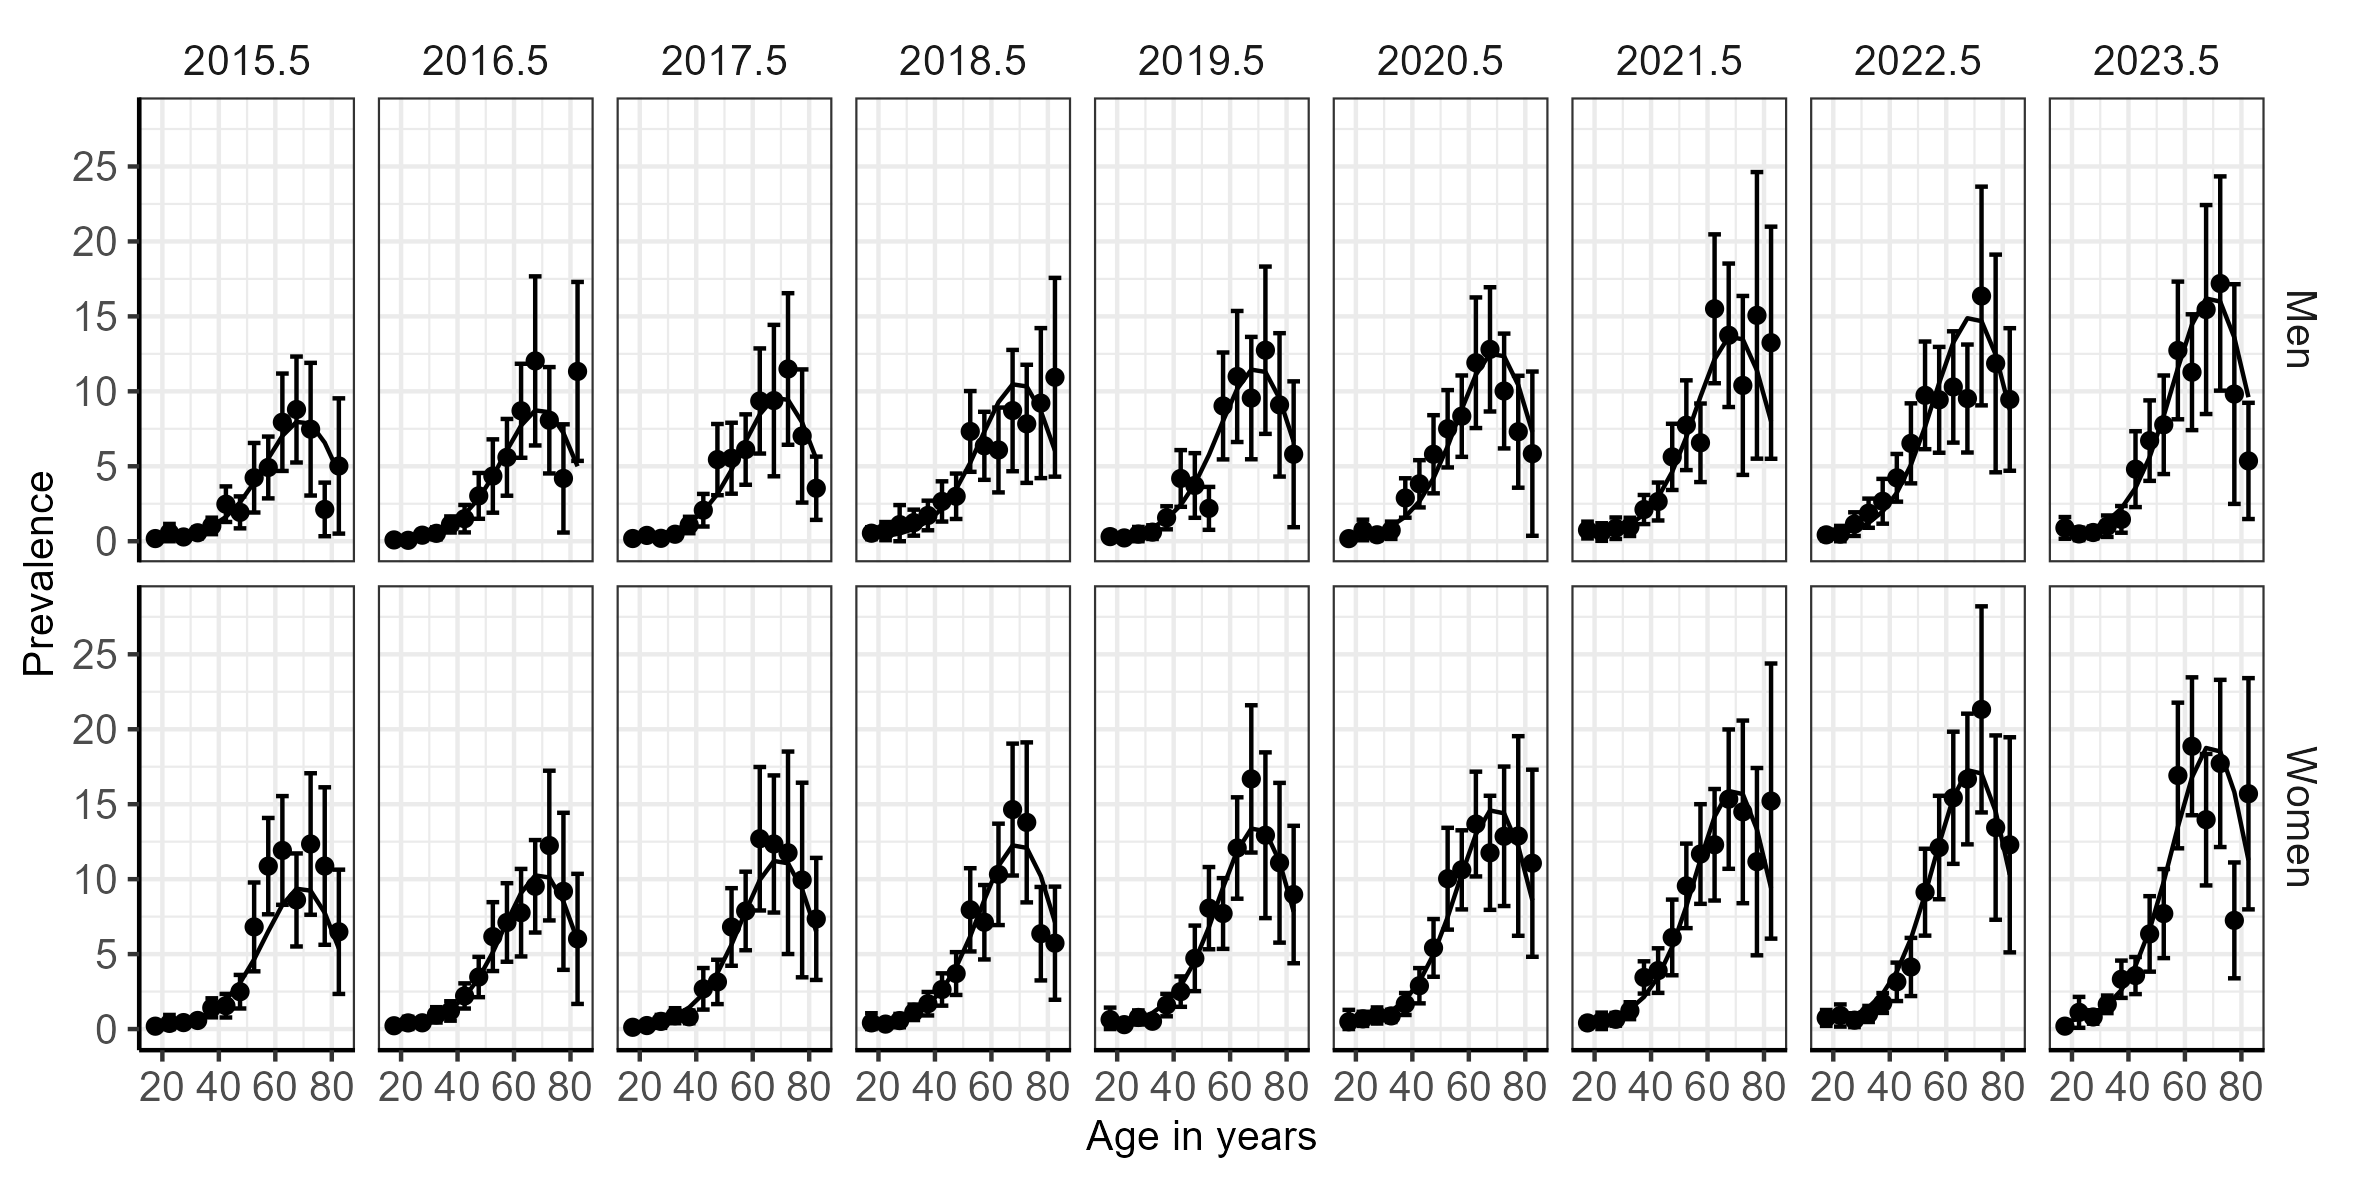
\includegraphics{plt.input_prev.png} \newpage{}
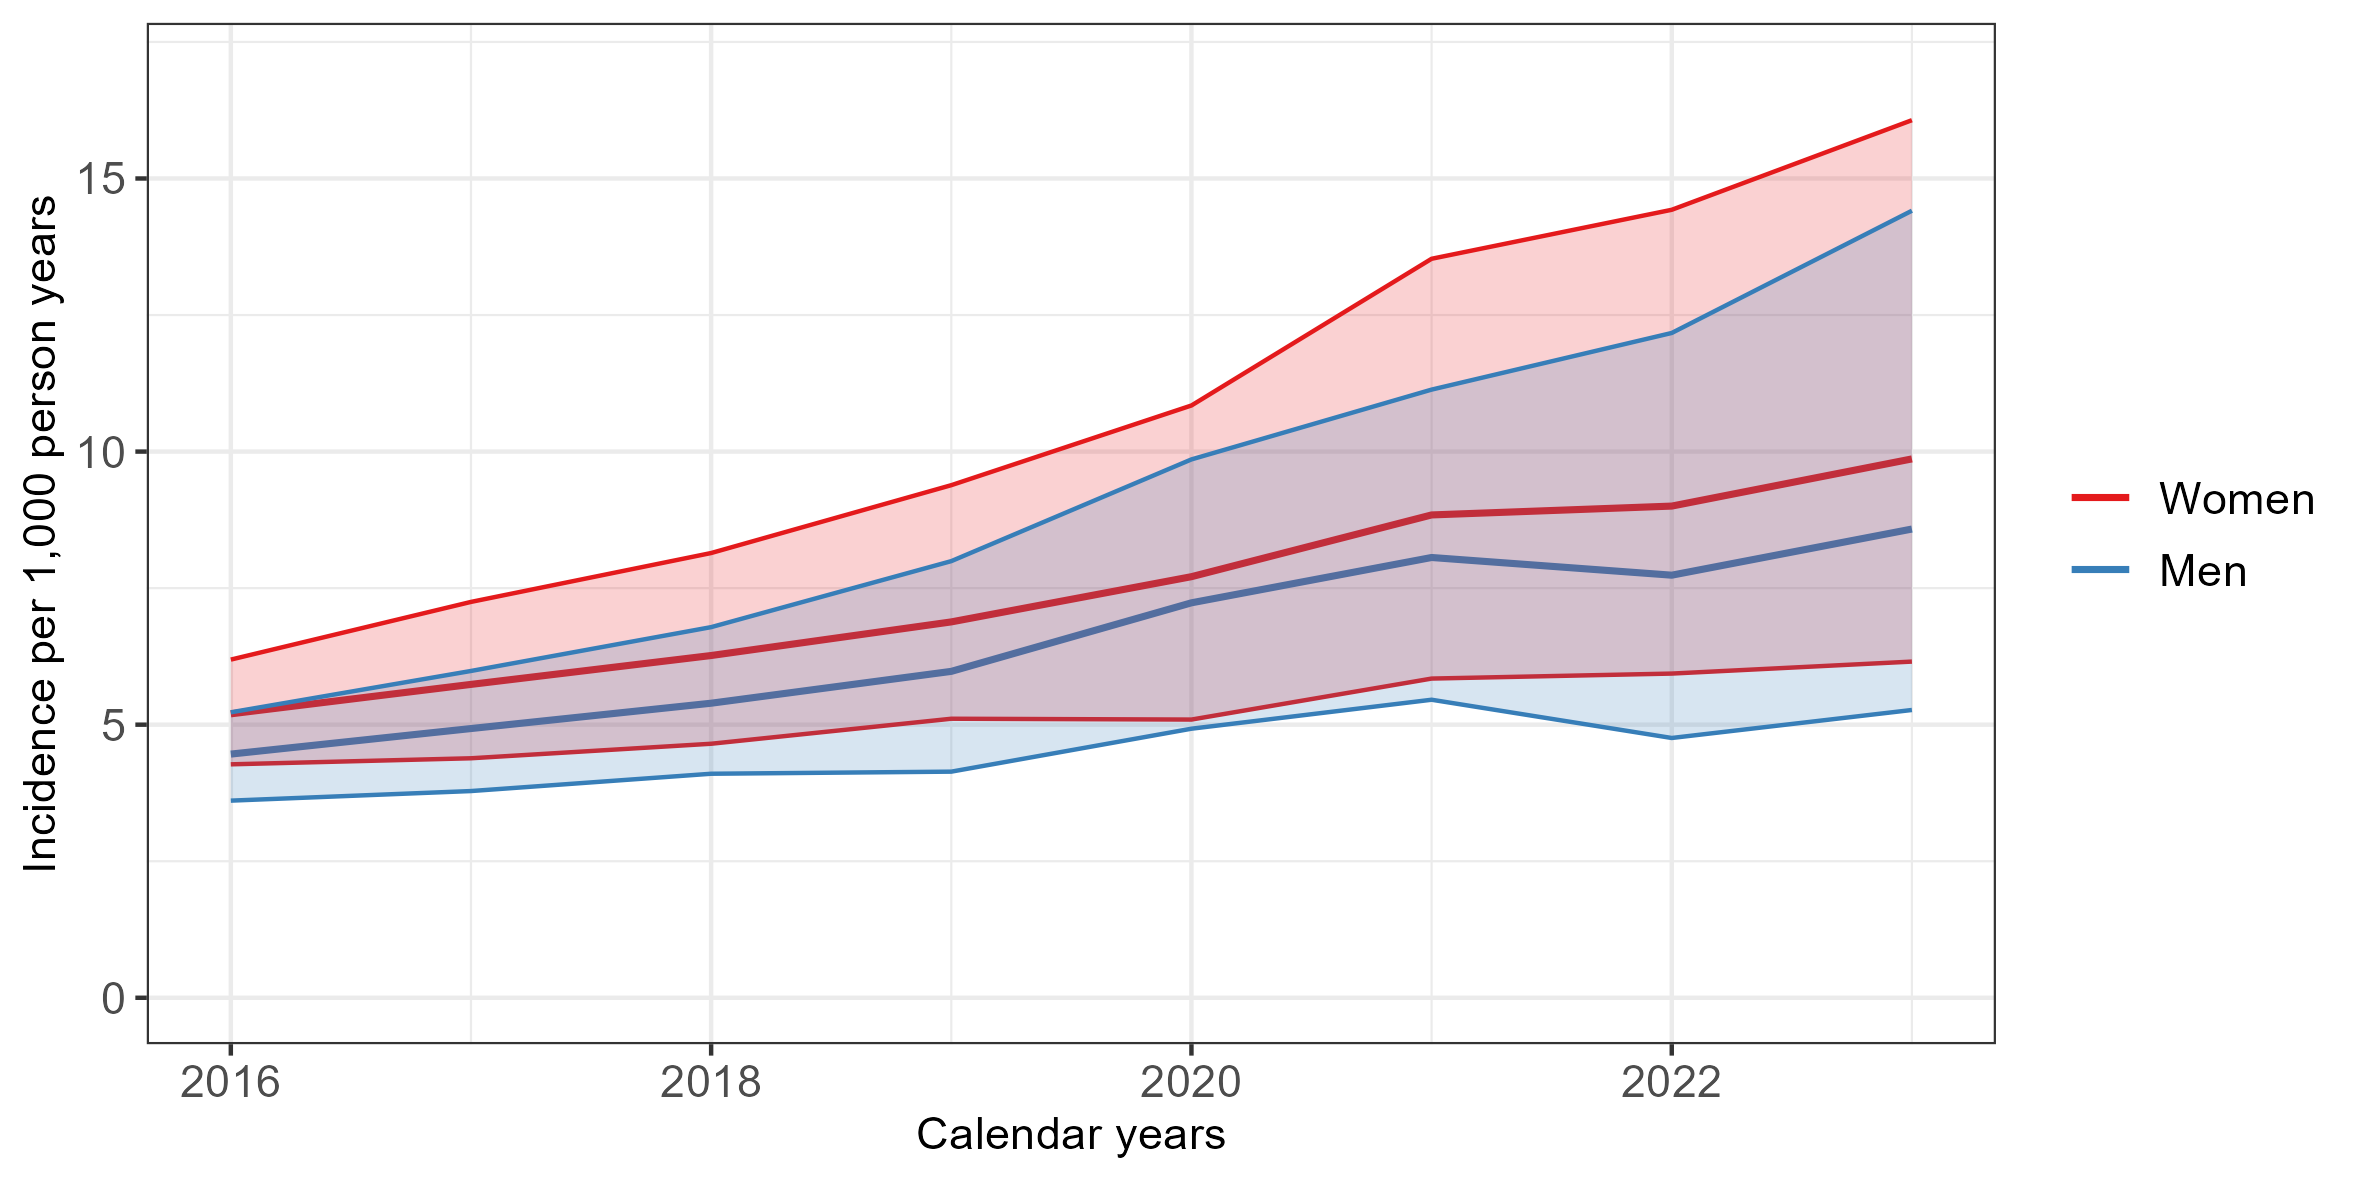
\includegraphics{plt.standardized.png}

\newpage{}

\subsection{Table 2. Age-standardized incidence rates of diabetes for
men and women in Peru for the years 2016-2023, and the temporal change
in incidence rates between 2016 and
2023}\label{table-2.-age-standardized-incidence-rates-of-diabetes-for-men-and-women-in-peru-for-the-years-2016-2023-and-the-temporal-change-in-incidence-rates-between-2016-and-2023}

\global\setlength{\Oldarrayrulewidth}{\arrayrulewidth}

\global\setlength{\Oldtabcolsep}{\tabcolsep}

\setlength{\tabcolsep}{2pt}

\renewcommand*{\arraystretch}{1.5}



\providecommand{\ascline}[3]{\noalign{\global\arrayrulewidth #1}\arrayrulecolor[HTML]{#2}\cline{#3}}

\begin{longtable*}[c]{|p{0.63in}|p{1.55in}|p{1.66in}|p{1.78in}|p{1.89in}}



\ascline{1.5pt}{666666}{1-5}

\multicolumn{1}{>{\raggedright}m{\dimexpr 0.63in+0\tabcolsep}}{\textcolor[HTML]{000000}{\fontsize{11}{11}\selectfont{\global\setmainfont{Arial}{Year}}}} & \multicolumn{1}{>{\raggedright}m{\dimexpr 1.55in+0\tabcolsep}}{\textcolor[HTML]{000000}{\fontsize{11}{11}\selectfont{\global\setmainfont{Arial}{Men\ –\ IR\ (95\%\ CI)}}}} & \multicolumn{1}{>{\raggedright}m{\dimexpr 1.66in+0\tabcolsep}}{\textcolor[HTML]{000000}{\fontsize{11}{11}\selectfont{\global\setmainfont{Arial}{Men\ –\ IRR\ (95\%\ CI)}}}} & \multicolumn{1}{>{\raggedright}m{\dimexpr 1.78in+0\tabcolsep}}{\textcolor[HTML]{000000}{\fontsize{11}{11}\selectfont{\global\setmainfont{Arial}{Women\ –\ IR\ (95\%\ CI)}}}} & \multicolumn{1}{>{\raggedright}m{\dimexpr 1.89in+0\tabcolsep}}{\textcolor[HTML]{000000}{\fontsize{11}{11}\selectfont{\global\setmainfont{Arial}{Women\ –\ IRR\ (95\%\ CI)}}}} \\

\ascline{1.5pt}{666666}{1-5}\endfirsthead 

\ascline{1.5pt}{666666}{1-5}

\multicolumn{1}{>{\raggedright}m{\dimexpr 0.63in+0\tabcolsep}}{\textcolor[HTML]{000000}{\fontsize{11}{11}\selectfont{\global\setmainfont{Arial}{Year}}}} & \multicolumn{1}{>{\raggedright}m{\dimexpr 1.55in+0\tabcolsep}}{\textcolor[HTML]{000000}{\fontsize{11}{11}\selectfont{\global\setmainfont{Arial}{Men\ –\ IR\ (95\%\ CI)}}}} & \multicolumn{1}{>{\raggedright}m{\dimexpr 1.66in+0\tabcolsep}}{\textcolor[HTML]{000000}{\fontsize{11}{11}\selectfont{\global\setmainfont{Arial}{Men\ –\ IRR\ (95\%\ CI)}}}} & \multicolumn{1}{>{\raggedright}m{\dimexpr 1.78in+0\tabcolsep}}{\textcolor[HTML]{000000}{\fontsize{11}{11}\selectfont{\global\setmainfont{Arial}{Women\ –\ IR\ (95\%\ CI)}}}} & \multicolumn{1}{>{\raggedright}m{\dimexpr 1.89in+0\tabcolsep}}{\textcolor[HTML]{000000}{\fontsize{11}{11}\selectfont{\global\setmainfont{Arial}{Women\ –\ IRR\ (95\%\ CI)}}}} \\

\ascline{1.5pt}{666666}{1-5}\endhead



\multicolumn{1}{>{\raggedright}m{\dimexpr 0.63in+0\tabcolsep}}{\textcolor[HTML]{000000}{\fontsize{11}{11}\selectfont{\global\setmainfont{Arial}{2016}}}} & \multicolumn{1}{>{\raggedright}m{\dimexpr 1.55in+0\tabcolsep}}{\textcolor[HTML]{000000}{\fontsize{11}{11}\selectfont{\global\setmainfont{Arial}{4.46\ (3.61–5.23)}}}} & \multicolumn{1}{>{\raggedright}m{\dimexpr 1.66in+0\tabcolsep}}{\textcolor[HTML]{000000}{\fontsize{11}{11}\selectfont{\global\setmainfont{Arial}{1.00\ (1.00–1.00)}}}} & \multicolumn{1}{>{\raggedright}m{\dimexpr 1.78in+0\tabcolsep}}{\textcolor[HTML]{000000}{\fontsize{11}{11}\selectfont{\global\setmainfont{Arial}{5.20\ (4.27–6.19)}}}} & \multicolumn{1}{>{\raggedright}m{\dimexpr 1.89in+0\tabcolsep}}{\textcolor[HTML]{000000}{\fontsize{11}{11}\selectfont{\global\setmainfont{Arial}{1.00\ (1.00–1.00)}}}} \\





\multicolumn{1}{>{\raggedright}m{\dimexpr 0.63in+0\tabcolsep}}{\textcolor[HTML]{000000}{\fontsize{11}{11}\selectfont{\global\setmainfont{Arial}{2017}}}} & \multicolumn{1}{>{\raggedright}m{\dimexpr 1.55in+0\tabcolsep}}{\textcolor[HTML]{000000}{\fontsize{11}{11}\selectfont{\global\setmainfont{Arial}{4.93\ (3.78–5.98)}}}} & \multicolumn{1}{>{\raggedright}m{\dimexpr 1.66in+0\tabcolsep}}{\textcolor[HTML]{000000}{\fontsize{11}{11}\selectfont{\global\setmainfont{Arial}{1.10\ (0.81–1.45)}}}} & \multicolumn{1}{>{\raggedright}m{\dimexpr 1.78in+0\tabcolsep}}{\textcolor[HTML]{000000}{\fontsize{11}{11}\selectfont{\global\setmainfont{Arial}{5.74\ (4.38–7.25)}}}} & \multicolumn{1}{>{\raggedright}m{\dimexpr 1.89in+0\tabcolsep}}{\textcolor[HTML]{000000}{\fontsize{11}{11}\selectfont{\global\setmainfont{Arial}{1.11\ (0.81–1.50)}}}} \\





\multicolumn{1}{>{\raggedright}m{\dimexpr 0.63in+0\tabcolsep}}{\textcolor[HTML]{000000}{\fontsize{11}{11}\selectfont{\global\setmainfont{Arial}{2018}}}} & \multicolumn{1}{>{\raggedright}m{\dimexpr 1.55in+0\tabcolsep}}{\textcolor[HTML]{000000}{\fontsize{11}{11}\selectfont{\global\setmainfont{Arial}{5.39\ (4.10–6.79)}}}} & \multicolumn{1}{>{\raggedright}m{\dimexpr 1.66in+0\tabcolsep}}{\textcolor[HTML]{000000}{\fontsize{11}{11}\selectfont{\global\setmainfont{Arial}{1.21\ (0.90–1.64)}}}} & \multicolumn{1}{>{\raggedright}m{\dimexpr 1.78in+0\tabcolsep}}{\textcolor[HTML]{000000}{\fontsize{11}{11}\selectfont{\global\setmainfont{Arial}{6.27\ (4.65–8.14)}}}} & \multicolumn{1}{>{\raggedright}m{\dimexpr 1.89in+0\tabcolsep}}{\textcolor[HTML]{000000}{\fontsize{11}{11}\selectfont{\global\setmainfont{Arial}{1.21\ (0.87–1.65)}}}} \\





\multicolumn{1}{>{\raggedright}m{\dimexpr 0.63in+0\tabcolsep}}{\textcolor[HTML]{000000}{\fontsize{11}{11}\selectfont{\global\setmainfont{Arial}{2019}}}} & \multicolumn{1}{>{\raggedright}m{\dimexpr 1.55in+0\tabcolsep}}{\textcolor[HTML]{000000}{\fontsize{11}{11}\selectfont{\global\setmainfont{Arial}{5.98\ (4.14–7.99)}}}} & \multicolumn{1}{>{\raggedright}m{\dimexpr 1.66in+0\tabcolsep}}{\textcolor[HTML]{000000}{\fontsize{11}{11}\selectfont{\global\setmainfont{Arial}{1.34\ (0.89–1.90)}}}} & \multicolumn{1}{>{\raggedright}m{\dimexpr 1.78in+0\tabcolsep}}{\textcolor[HTML]{000000}{\fontsize{11}{11}\selectfont{\global\setmainfont{Arial}{6.88\ (5.11–9.38)}}}} & \multicolumn{1}{>{\raggedright}m{\dimexpr 1.89in+0\tabcolsep}}{\textcolor[HTML]{000000}{\fontsize{11}{11}\selectfont{\global\setmainfont{Arial}{1.34\ (0.94–1.89)}}}} \\





\multicolumn{1}{>{\raggedright}m{\dimexpr 0.63in+0\tabcolsep}}{\textcolor[HTML]{000000}{\fontsize{11}{11}\selectfont{\global\setmainfont{Arial}{2020}}}} & \multicolumn{1}{>{\raggedright}m{\dimexpr 1.55in+0\tabcolsep}}{\textcolor[HTML]{000000}{\fontsize{11}{11}\selectfont{\global\setmainfont{Arial}{7.23\ (4.93–9.86)}}}} & \multicolumn{1}{>{\raggedright}m{\dimexpr 1.66in+0\tabcolsep}}{\textcolor[HTML]{000000}{\fontsize{11}{11}\selectfont{\global\setmainfont{Arial}{1.64\ (1.08–2.33)}}}} & \multicolumn{1}{>{\raggedright}m{\dimexpr 1.78in+0\tabcolsep}}{\textcolor[HTML]{000000}{\fontsize{11}{11}\selectfont{\global\setmainfont{Arial}{7.71\ (5.09–10.84)}}}} & \multicolumn{1}{>{\raggedright}m{\dimexpr 1.89in+0\tabcolsep}}{\textcolor[HTML]{000000}{\fontsize{11}{11}\selectfont{\global\setmainfont{Arial}{1.49\ (0.97–2.22)}}}} \\





\multicolumn{1}{>{\raggedright}m{\dimexpr 0.63in+0\tabcolsep}}{\textcolor[HTML]{000000}{\fontsize{11}{11}\selectfont{\global\setmainfont{Arial}{2021}}}} & \multicolumn{1}{>{\raggedright}m{\dimexpr 1.55in+0\tabcolsep}}{\textcolor[HTML]{000000}{\fontsize{11}{11}\selectfont{\global\setmainfont{Arial}{8.06\ (5.46–11.13)}}}} & \multicolumn{1}{>{\raggedright}m{\dimexpr 1.66in+0\tabcolsep}}{\textcolor[HTML]{000000}{\fontsize{11}{11}\selectfont{\global\setmainfont{Arial}{1.81\ (1.19–2.64)}}}} & \multicolumn{1}{>{\raggedright}m{\dimexpr 1.78in+0\tabcolsep}}{\textcolor[HTML]{000000}{\fontsize{11}{11}\selectfont{\global\setmainfont{Arial}{8.84\ (5.84–13.53)}}}} & \multicolumn{1}{>{\raggedright}m{\dimexpr 1.89in+0\tabcolsep}}{\textcolor[HTML]{000000}{\fontsize{11}{11}\selectfont{\global\setmainfont{Arial}{1.71\ (1.13–2.69)}}}} \\





\multicolumn{1}{>{\raggedright}m{\dimexpr 0.63in+0\tabcolsep}}{\textcolor[HTML]{000000}{\fontsize{11}{11}\selectfont{\global\setmainfont{Arial}{2022}}}} & \multicolumn{1}{>{\raggedright}m{\dimexpr 1.55in+0\tabcolsep}}{\textcolor[HTML]{000000}{\fontsize{11}{11}\selectfont{\global\setmainfont{Arial}{7.74\ (4.76–12.17)}}}} & \multicolumn{1}{>{\raggedright}m{\dimexpr 1.66in+0\tabcolsep}}{\textcolor[HTML]{000000}{\fontsize{11}{11}\selectfont{\global\setmainfont{Arial}{1.76\ (1.07–2.79)}}}} & \multicolumn{1}{>{\raggedright}m{\dimexpr 1.78in+0\tabcolsep}}{\textcolor[HTML]{000000}{\fontsize{11}{11}\selectfont{\global\setmainfont{Arial}{9.00\ (5.94–14.43)}}}} & \multicolumn{1}{>{\raggedright}m{\dimexpr 1.89in+0\tabcolsep}}{\textcolor[HTML]{000000}{\fontsize{11}{11}\selectfont{\global\setmainfont{Arial}{1.74\ (1.13–2.89)}}}} \\





\multicolumn{1}{>{\raggedright}m{\dimexpr 0.63in+0\tabcolsep}}{\textcolor[HTML]{000000}{\fontsize{11}{11}\selectfont{\global\setmainfont{Arial}{2023}}}} & \multicolumn{1}{>{\raggedright}m{\dimexpr 1.55in+0\tabcolsep}}{\textcolor[HTML]{000000}{\fontsize{11}{11}\selectfont{\global\setmainfont{Arial}{8.58\ (5.27–14.41)}}}} & \multicolumn{1}{>{\raggedright}m{\dimexpr 1.66in+0\tabcolsep}}{\textcolor[HTML]{000000}{\fontsize{11}{11}\selectfont{\global\setmainfont{Arial}{1.93\ (1.14–3.24)}}}} & \multicolumn{1}{>{\raggedright}m{\dimexpr 1.78in+0\tabcolsep}}{\textcolor[HTML]{000000}{\fontsize{11}{11}\selectfont{\global\setmainfont{Arial}{9.87\ (6.16–16.07)}}}} & \multicolumn{1}{>{\raggedright}m{\dimexpr 1.89in+0\tabcolsep}}{\textcolor[HTML]{000000}{\fontsize{11}{11}\selectfont{\global\setmainfont{Arial}{1.92\ (1.15–3.16)}}}} \\

\ascline{1.5pt}{666666}{1-5}



\end{longtable*}



\arrayrulecolor[HTML]{000000}

\global\setlength{\arrayrulewidth}{\Oldarrayrulewidth}

\global\setlength{\tabcolsep}{\Oldtabcolsep}

\renewcommand*{\arraystretch}{1}

\newpage{} 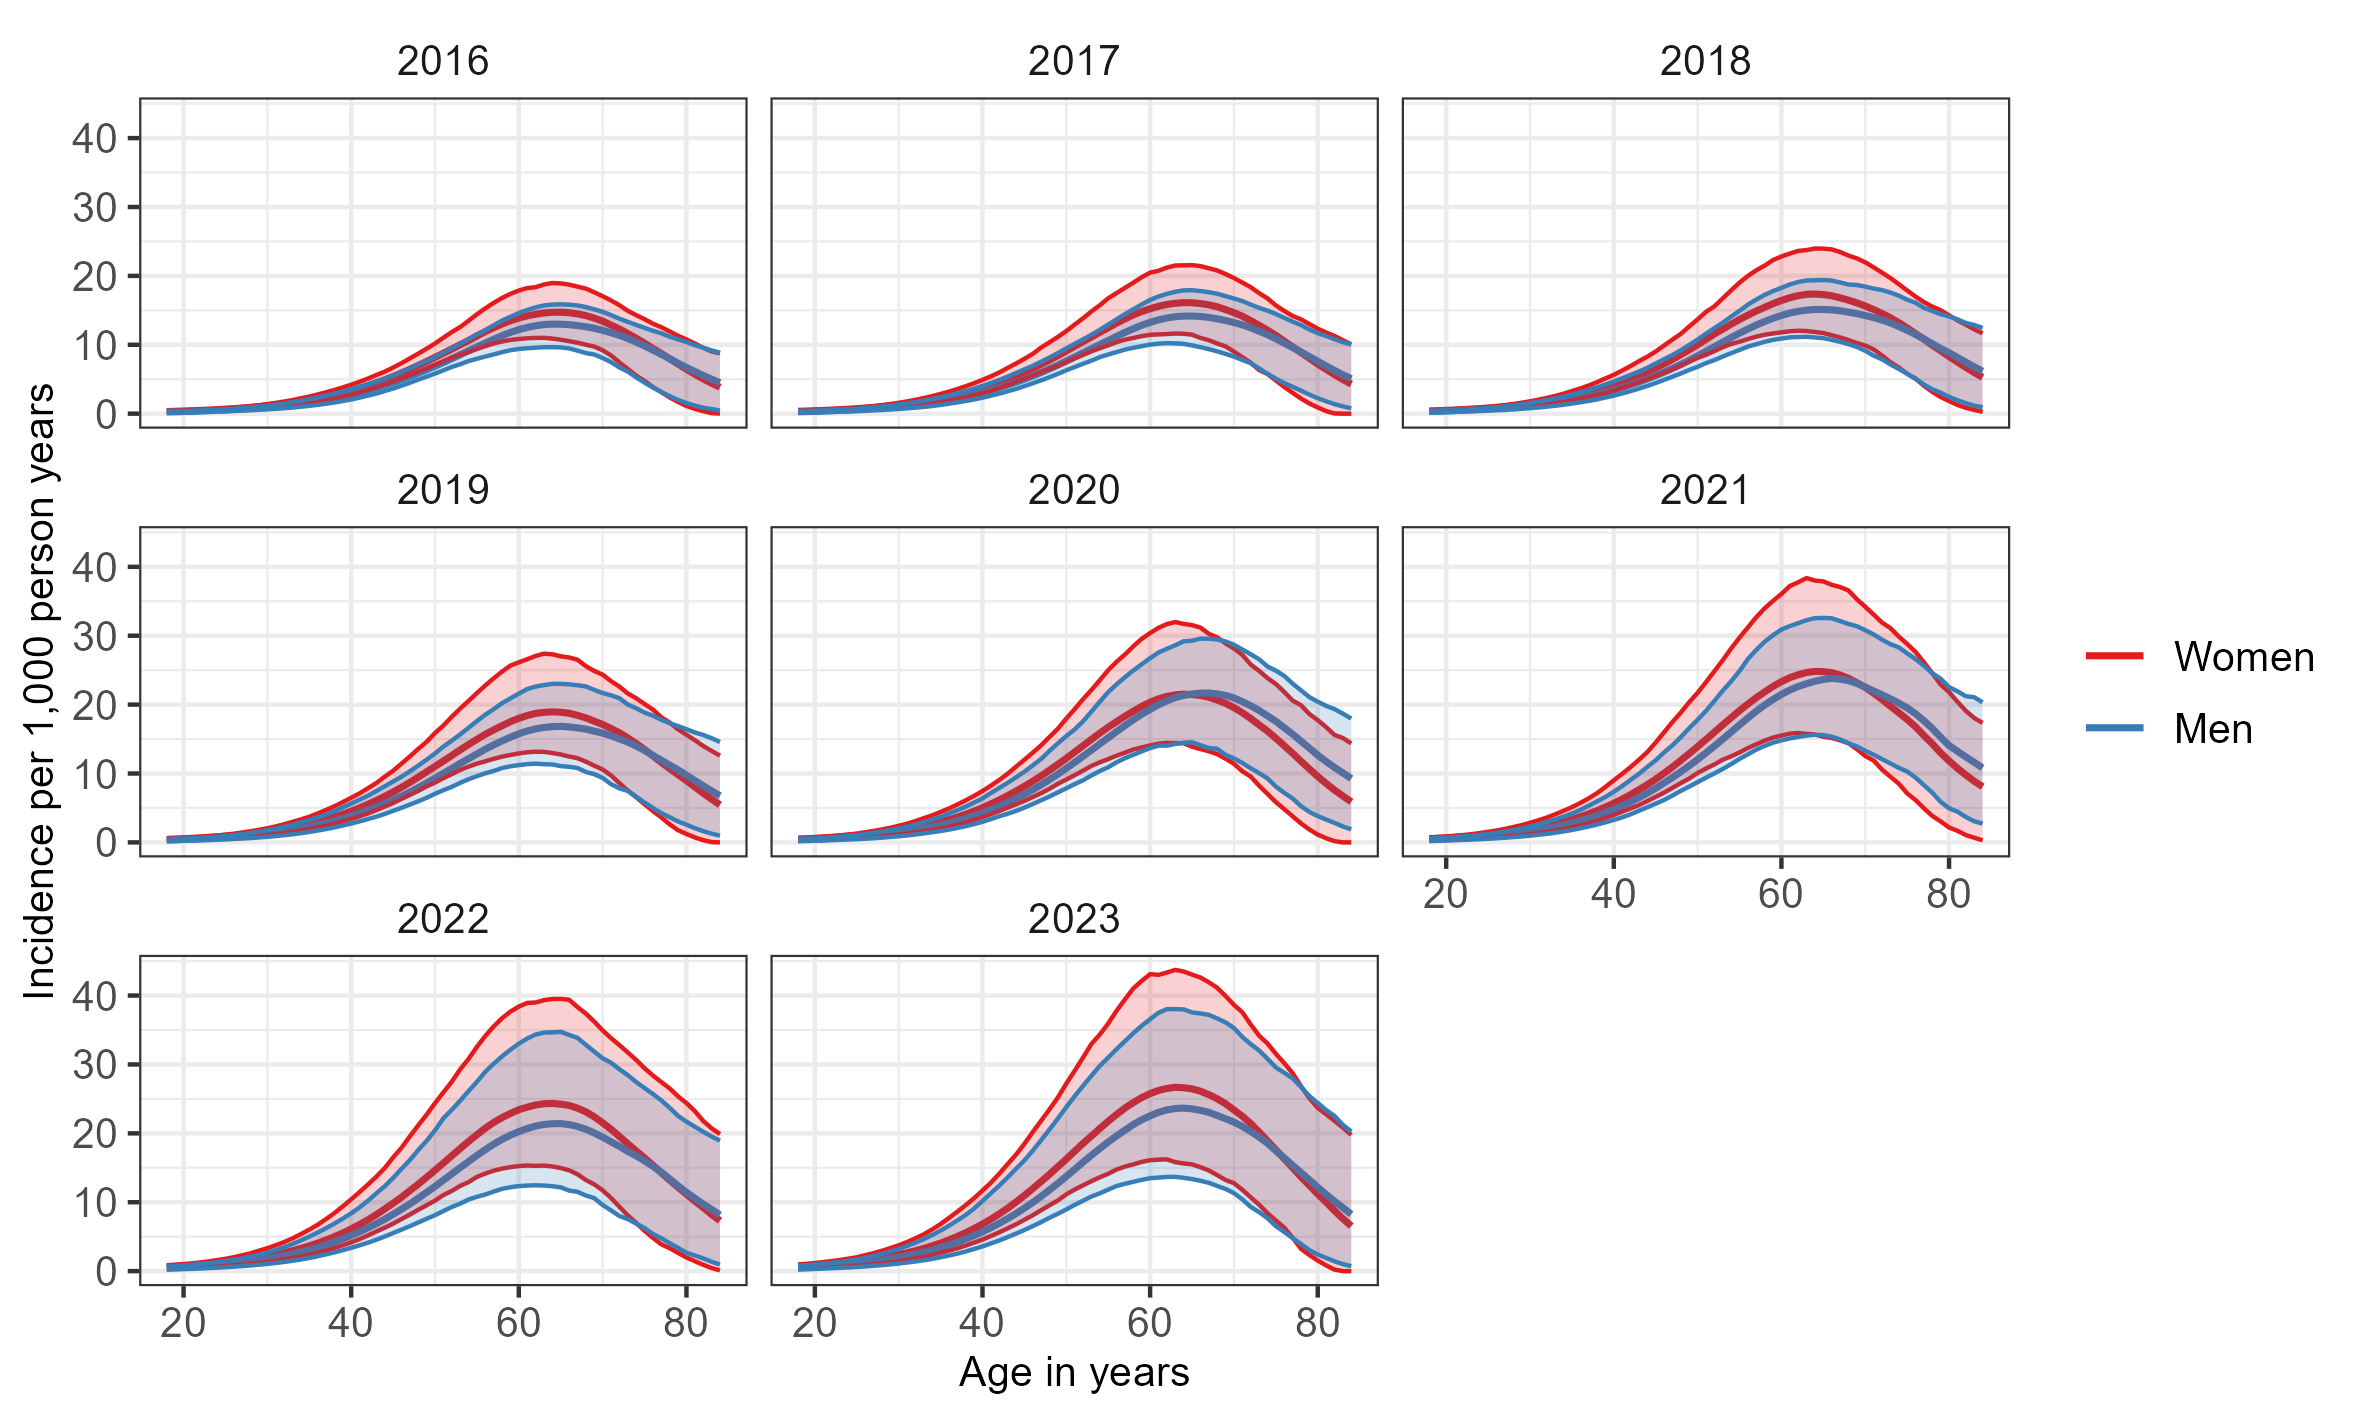
\includegraphics{plt.inc_age.png} \newpage{}

\subsection{Table 3. Age and sex-specific incidence rates of diabetes in
Peru for the years 2016-2023, and the temporal change in incidence rates
between 2016 and
2023}\label{table-3.-age-and-sex-specific-incidence-rates-of-diabetes-in-peru-for-the-years-2016-2023-and-the-temporal-change-in-incidence-rates-between-2016-and-2023}

\global\setlength{\Oldarrayrulewidth}{\arrayrulewidth}

\global\setlength{\Oldtabcolsep}{\tabcolsep}

\setlength{\tabcolsep}{2pt}

\renewcommand*{\arraystretch}{1.5}



\providecommand{\ascline}[3]{\noalign{\global\arrayrulewidth #1}\arrayrulecolor[HTML]{#2}\cline{#3}}

\begin{longtable*}[c]{|p{0.54in}|p{0.63in}|p{1.66in}|p{1.66in}|p{1.78in}|p{1.89in}}



\ascline{1.5pt}{666666}{1-6}

\multicolumn{1}{>{\raggedright}m{\dimexpr 0.54in+0\tabcolsep}}{\textcolor[HTML]{000000}{\fontsize{11}{11}\selectfont{\global\setmainfont{Arial}{age}}}} & \multicolumn{1}{>{\raggedright}m{\dimexpr 0.63in+0\tabcolsep}}{\textcolor[HTML]{000000}{\fontsize{11}{11}\selectfont{\global\setmainfont{Arial}{Year}}}} & \multicolumn{1}{>{\raggedright}m{\dimexpr 1.66in+0\tabcolsep}}{\textcolor[HTML]{000000}{\fontsize{11}{11}\selectfont{\global\setmainfont{Arial}{Men\ –\ IR\ (95\%\ CI)}}}} & \multicolumn{1}{>{\raggedright}m{\dimexpr 1.66in+0\tabcolsep}}{\textcolor[HTML]{000000}{\fontsize{11}{11}\selectfont{\global\setmainfont{Arial}{Men\ –\ IRR\ (95\%\ CI)}}}} & \multicolumn{1}{>{\raggedright}m{\dimexpr 1.78in+0\tabcolsep}}{\textcolor[HTML]{000000}{\fontsize{11}{11}\selectfont{\global\setmainfont{Arial}{Women\ –\ IR\ (95\%\ CI)}}}} & \multicolumn{1}{>{\raggedright}m{\dimexpr 1.89in+0\tabcolsep}}{\textcolor[HTML]{000000}{\fontsize{11}{11}\selectfont{\global\setmainfont{Arial}{Women\ –\ IRR\ (95\%\ CI)}}}} \\

\ascline{1.5pt}{666666}{1-6}\endfirsthead 

\ascline{1.5pt}{666666}{1-6}

\multicolumn{1}{>{\raggedright}m{\dimexpr 0.54in+0\tabcolsep}}{\textcolor[HTML]{000000}{\fontsize{11}{11}\selectfont{\global\setmainfont{Arial}{age}}}} & \multicolumn{1}{>{\raggedright}m{\dimexpr 0.63in+0\tabcolsep}}{\textcolor[HTML]{000000}{\fontsize{11}{11}\selectfont{\global\setmainfont{Arial}{Year}}}} & \multicolumn{1}{>{\raggedright}m{\dimexpr 1.66in+0\tabcolsep}}{\textcolor[HTML]{000000}{\fontsize{11}{11}\selectfont{\global\setmainfont{Arial}{Men\ –\ IR\ (95\%\ CI)}}}} & \multicolumn{1}{>{\raggedright}m{\dimexpr 1.66in+0\tabcolsep}}{\textcolor[HTML]{000000}{\fontsize{11}{11}\selectfont{\global\setmainfont{Arial}{Men\ –\ IRR\ (95\%\ CI)}}}} & \multicolumn{1}{>{\raggedright}m{\dimexpr 1.78in+0\tabcolsep}}{\textcolor[HTML]{000000}{\fontsize{11}{11}\selectfont{\global\setmainfont{Arial}{Women\ –\ IR\ (95\%\ CI)}}}} & \multicolumn{1}{>{\raggedright}m{\dimexpr 1.89in+0\tabcolsep}}{\textcolor[HTML]{000000}{\fontsize{11}{11}\selectfont{\global\setmainfont{Arial}{Women\ –\ IRR\ (95\%\ CI)}}}} \\

\ascline{1.5pt}{666666}{1-6}\endhead



\multicolumn{1}{>{\raggedright}m{\dimexpr 0.54in+0\tabcolsep}}{\textcolor[HTML]{000000}{\fontsize{11}{11}\selectfont{\global\setmainfont{Arial}{20}}}} & \multicolumn{1}{>{\raggedright}m{\dimexpr 0.63in+0\tabcolsep}}{\textcolor[HTML]{000000}{\fontsize{11}{11}\selectfont{\global\setmainfont{Arial}{2016}}}} & \multicolumn{1}{>{\raggedright}m{\dimexpr 1.66in+0\tabcolsep}}{\textcolor[HTML]{000000}{\fontsize{11}{11}\selectfont{\global\setmainfont{Arial}{0.31\ (0.18–0.40)}}}} & \multicolumn{1}{>{\raggedright}m{\dimexpr 1.66in+0\tabcolsep}}{\textcolor[HTML]{000000}{\fontsize{11}{11}\selectfont{\global\setmainfont{Arial}{1.00\ (1.00–1.00)}}}} & \multicolumn{1}{>{\raggedright}m{\dimexpr 1.78in+0\tabcolsep}}{\textcolor[HTML]{000000}{\fontsize{11}{11}\selectfont{\global\setmainfont{Arial}{0.38\ (0.21–0.47)}}}} & \multicolumn{1}{>{\raggedright}m{\dimexpr 1.89in+0\tabcolsep}}{\textcolor[HTML]{000000}{\fontsize{11}{11}\selectfont{\global\setmainfont{Arial}{1.00\ (1.00–1.00)}}}} \\





\multicolumn{1}{>{\raggedright}m{\dimexpr 0.54in+0\tabcolsep}}{\textcolor[HTML]{000000}{\fontsize{11}{11}\selectfont{\global\setmainfont{Arial}{20}}}} & \multicolumn{1}{>{\raggedright}m{\dimexpr 0.63in+0\tabcolsep}}{\textcolor[HTML]{000000}{\fontsize{11}{11}\selectfont{\global\setmainfont{Arial}{2023}}}} & \multicolumn{1}{>{\raggedright}m{\dimexpr 1.66in+0\tabcolsep}}{\textcolor[HTML]{000000}{\fontsize{11}{11}\selectfont{\global\setmainfont{Arial}{0.68\ (0.31–0.96)}}}} & \multicolumn{1}{>{\raggedright}m{\dimexpr 1.66in+0\tabcolsep}}{\textcolor[HTML]{000000}{\fontsize{11}{11}\selectfont{\global\setmainfont{Arial}{2.18\ (1.00–4.21)}}}} & \multicolumn{1}{>{\raggedright}m{\dimexpr 1.78in+0\tabcolsep}}{\textcolor[HTML]{000000}{\fontsize{11}{11}\selectfont{\global\setmainfont{Arial}{0.83\ (0.39–1.18)}}}} & \multicolumn{1}{>{\raggedright}m{\dimexpr 1.89in+0\tabcolsep}}{\textcolor[HTML]{000000}{\fontsize{11}{11}\selectfont{\global\setmainfont{Arial}{2.16\ (1.03–4.28)}}}} \\





\multicolumn{1}{>{\raggedright}m{\dimexpr 0.54in+0\tabcolsep}}{\textcolor[HTML]{000000}{\fontsize{11}{11}\selectfont{\global\setmainfont{Arial}{30}}}} & \multicolumn{1}{>{\raggedright}m{\dimexpr 0.63in+0\tabcolsep}}{\textcolor[HTML]{000000}{\fontsize{11}{11}\selectfont{\global\setmainfont{Arial}{2016}}}} & \multicolumn{1}{>{\raggedright}m{\dimexpr 1.66in+0\tabcolsep}}{\textcolor[HTML]{000000}{\fontsize{11}{11}\selectfont{\global\setmainfont{Arial}{0.96\ (0.62–1.17)}}}} & \multicolumn{1}{>{\raggedright}m{\dimexpr 1.66in+0\tabcolsep}}{\textcolor[HTML]{000000}{\fontsize{11}{11}\selectfont{\global\setmainfont{Arial}{1.00\ (1.00–1.00)}}}} & \multicolumn{1}{>{\raggedright}m{\dimexpr 1.78in+0\tabcolsep}}{\textcolor[HTML]{000000}{\fontsize{11}{11}\selectfont{\global\setmainfont{Arial}{1.14\ (0.84–1.39)}}}} & \multicolumn{1}{>{\raggedright}m{\dimexpr 1.89in+0\tabcolsep}}{\textcolor[HTML]{000000}{\fontsize{11}{11}\selectfont{\global\setmainfont{Arial}{1.00\ (1.00–1.00)}}}} \\





\multicolumn{1}{>{\raggedright}m{\dimexpr 0.54in+0\tabcolsep}}{\textcolor[HTML]{000000}{\fontsize{11}{11}\selectfont{\global\setmainfont{Arial}{30}}}} & \multicolumn{1}{>{\raggedright}m{\dimexpr 0.63in+0\tabcolsep}}{\textcolor[HTML]{000000}{\fontsize{11}{11}\selectfont{\global\setmainfont{Arial}{2023}}}} & \multicolumn{1}{>{\raggedright}m{\dimexpr 1.66in+0\tabcolsep}}{\textcolor[HTML]{000000}{\fontsize{11}{11}\selectfont{\global\setmainfont{Arial}{2.00\ (1.10–3.23)}}}} & \multicolumn{1}{>{\raggedright}m{\dimexpr 1.66in+0\tabcolsep}}{\textcolor[HTML]{000000}{\fontsize{11}{11}\selectfont{\global\setmainfont{Arial}{2.13\ (1.17–3.76)}}}} & \multicolumn{1}{>{\raggedright}m{\dimexpr 1.78in+0\tabcolsep}}{\textcolor[HTML]{000000}{\fontsize{11}{11}\selectfont{\global\setmainfont{Arial}{2.39\ (1.44–3.75)}}}} & \multicolumn{1}{>{\raggedright}m{\dimexpr 1.89in+0\tabcolsep}}{\textcolor[HTML]{000000}{\fontsize{11}{11}\selectfont{\global\setmainfont{Arial}{2.11\ (1.25–3.52)}}}} \\





\multicolumn{1}{>{\raggedright}m{\dimexpr 0.54in+0\tabcolsep}}{\textcolor[HTML]{000000}{\fontsize{11}{11}\selectfont{\global\setmainfont{Arial}{40}}}} & \multicolumn{1}{>{\raggedright}m{\dimexpr 0.63in+0\tabcolsep}}{\textcolor[HTML]{000000}{\fontsize{11}{11}\selectfont{\global\setmainfont{Arial}{2016}}}} & \multicolumn{1}{>{\raggedright}m{\dimexpr 1.66in+0\tabcolsep}}{\textcolor[HTML]{000000}{\fontsize{11}{11}\selectfont{\global\setmainfont{Arial}{2.79\ (2.06–3.55)}}}} & \multicolumn{1}{>{\raggedright}m{\dimexpr 1.66in+0\tabcolsep}}{\textcolor[HTML]{000000}{\fontsize{11}{11}\selectfont{\global\setmainfont{Arial}{1.00\ (1.00–1.00)}}}} & \multicolumn{1}{>{\raggedright}m{\dimexpr 1.78in+0\tabcolsep}}{\textcolor[HTML]{000000}{\fontsize{11}{11}\selectfont{\global\setmainfont{Arial}{3.32\ (2.76–4.20)}}}} & \multicolumn{1}{>{\raggedright}m{\dimexpr 1.89in+0\tabcolsep}}{\textcolor[HTML]{000000}{\fontsize{11}{11}\selectfont{\global\setmainfont{Arial}{1.00\ (1.00–1.00)}}}} \\





\multicolumn{1}{>{\raggedright}m{\dimexpr 0.54in+0\tabcolsep}}{\textcolor[HTML]{000000}{\fontsize{11}{11}\selectfont{\global\setmainfont{Arial}{40}}}} & \multicolumn{1}{>{\raggedright}m{\dimexpr 0.63in+0\tabcolsep}}{\textcolor[HTML]{000000}{\fontsize{11}{11}\selectfont{\global\setmainfont{Arial}{2023}}}} & \multicolumn{1}{>{\raggedright}m{\dimexpr 1.66in+0\tabcolsep}}{\textcolor[HTML]{000000}{\fontsize{11}{11}\selectfont{\global\setmainfont{Arial}{5.71\ (3.58–10.19)}}}} & \multicolumn{1}{>{\raggedright}m{\dimexpr 1.66in+0\tabcolsep}}{\textcolor[HTML]{000000}{\fontsize{11}{11}\selectfont{\global\setmainfont{Arial}{2.06\ (1.25–3.71)}}}} & \multicolumn{1}{>{\raggedright}m{\dimexpr 1.78in+0\tabcolsep}}{\textcolor[HTML]{000000}{\fontsize{11}{11}\selectfont{\global\setmainfont{Arial}{6.83\ (4.58–11.70)}}}} & \multicolumn{1}{>{\raggedright}m{\dimexpr 1.89in+0\tabcolsep}}{\textcolor[HTML]{000000}{\fontsize{11}{11}\selectfont{\global\setmainfont{Arial}{2.07\ (1.31–3.52)}}}} \\





\multicolumn{1}{>{\raggedright}m{\dimexpr 0.54in+0\tabcolsep}}{\textcolor[HTML]{000000}{\fontsize{11}{11}\selectfont{\global\setmainfont{Arial}{50}}}} & \multicolumn{1}{>{\raggedright}m{\dimexpr 0.63in+0\tabcolsep}}{\textcolor[HTML]{000000}{\fontsize{11}{11}\selectfont{\global\setmainfont{Arial}{2016}}}} & \multicolumn{1}{>{\raggedright}m{\dimexpr 1.66in+0\tabcolsep}}{\textcolor[HTML]{000000}{\fontsize{11}{11}\selectfont{\global\setmainfont{Arial}{6.89\ (5.82–8.23)}}}} & \multicolumn{1}{>{\raggedright}m{\dimexpr 1.66in+0\tabcolsep}}{\textcolor[HTML]{000000}{\fontsize{11}{11}\selectfont{\global\setmainfont{Arial}{1.00\ (1.00–1.00)}}}} & \multicolumn{1}{>{\raggedright}m{\dimexpr 1.78in+0\tabcolsep}}{\textcolor[HTML]{000000}{\fontsize{11}{11}\selectfont{\global\setmainfont{Arial}{8.17\ (7.07–10.18)}}}} & \multicolumn{1}{>{\raggedright}m{\dimexpr 1.89in+0\tabcolsep}}{\textcolor[HTML]{000000}{\fontsize{11}{11}\selectfont{\global\setmainfont{Arial}{1.00\ (1.00–1.00)}}}} \\





\multicolumn{1}{>{\raggedright}m{\dimexpr 0.54in+0\tabcolsep}}{\textcolor[HTML]{000000}{\fontsize{11}{11}\selectfont{\global\setmainfont{Arial}{50}}}} & \multicolumn{1}{>{\raggedright}m{\dimexpr 0.63in+0\tabcolsep}}{\textcolor[HTML]{000000}{\fontsize{11}{11}\selectfont{\global\setmainfont{Arial}{2023}}}} & \multicolumn{1}{>{\raggedright}m{\dimexpr 1.66in+0\tabcolsep}}{\textcolor[HTML]{000000}{\fontsize{11}{11}\selectfont{\global\setmainfont{Arial}{13.74\ (8.96–23.81)}}}} & \multicolumn{1}{>{\raggedright}m{\dimexpr 1.66in+0\tabcolsep}}{\textcolor[HTML]{000000}{\fontsize{11}{11}\selectfont{\global\setmainfont{Arial}{1.99\ (1.29–3.46)}}}} & \multicolumn{1}{>{\raggedright}m{\dimexpr 1.78in+0\tabcolsep}}{\textcolor[HTML]{000000}{\fontsize{11}{11}\selectfont{\global\setmainfont{Arial}{16.26\ (11.14–27.22)}}}} & \multicolumn{1}{>{\raggedright}m{\dimexpr 1.89in+0\tabcolsep}}{\textcolor[HTML]{000000}{\fontsize{11}{11}\selectfont{\global\setmainfont{Arial}{1.99\ (1.29–3.40)}}}} \\





\multicolumn{1}{>{\raggedright}m{\dimexpr 0.54in+0\tabcolsep}}{\textcolor[HTML]{000000}{\fontsize{11}{11}\selectfont{\global\setmainfont{Arial}{60}}}} & \multicolumn{1}{>{\raggedright}m{\dimexpr 0.63in+0\tabcolsep}}{\textcolor[HTML]{000000}{\fontsize{11}{11}\selectfont{\global\setmainfont{Arial}{2016}}}} & \multicolumn{1}{>{\raggedright}m{\dimexpr 1.66in+0\tabcolsep}}{\textcolor[HTML]{000000}{\fontsize{11}{11}\selectfont{\global\setmainfont{Arial}{12.20\ (9.39–14.60)}}}} & \multicolumn{1}{>{\raggedright}m{\dimexpr 1.66in+0\tabcolsep}}{\textcolor[HTML]{000000}{\fontsize{11}{11}\selectfont{\global\setmainfont{Arial}{1.00\ (1.00–1.00)}}}} & \multicolumn{1}{>{\raggedright}m{\dimexpr 1.78in+0\tabcolsep}}{\textcolor[HTML]{000000}{\fontsize{11}{11}\selectfont{\global\setmainfont{Arial}{13.88\ (10.83–17.87)}}}} & \multicolumn{1}{>{\raggedright}m{\dimexpr 1.89in+0\tabcolsep}}{\textcolor[HTML]{000000}{\fontsize{11}{11}\selectfont{\global\setmainfont{Arial}{1.00\ (1.00–1.00)}}}} \\





\multicolumn{1}{>{\raggedright}m{\dimexpr 0.54in+0\tabcolsep}}{\textcolor[HTML]{000000}{\fontsize{11}{11}\selectfont{\global\setmainfont{Arial}{60}}}} & \multicolumn{1}{>{\raggedright}m{\dimexpr 0.63in+0\tabcolsep}}{\textcolor[HTML]{000000}{\fontsize{11}{11}\selectfont{\global\setmainfont{Arial}{2023}}}} & \multicolumn{1}{>{\raggedright}m{\dimexpr 1.66in+0\tabcolsep}}{\textcolor[HTML]{000000}{\fontsize{11}{11}\selectfont{\global\setmainfont{Arial}{22.54\ (13.49–36.57)}}}} & \multicolumn{1}{>{\raggedright}m{\dimexpr 1.66in+0\tabcolsep}}{\textcolor[HTML]{000000}{\fontsize{11}{11}\selectfont{\global\setmainfont{Arial}{1.86\ (1.13–3.22)}}}} & \multicolumn{1}{>{\raggedright}m{\dimexpr 1.78in+0\tabcolsep}}{\textcolor[HTML]{000000}{\fontsize{11}{11}\selectfont{\global\setmainfont{Arial}{25.76\ (16.10–43.11)}}}} & \multicolumn{1}{>{\raggedright}m{\dimexpr 1.89in+0\tabcolsep}}{\textcolor[HTML]{000000}{\fontsize{11}{11}\selectfont{\global\setmainfont{Arial}{1.87\ (1.09–3.18)}}}} \\





\multicolumn{1}{>{\raggedright}m{\dimexpr 0.54in+0\tabcolsep}}{\textcolor[HTML]{000000}{\fontsize{11}{11}\selectfont{\global\setmainfont{Arial}{70}}}} & \multicolumn{1}{>{\raggedright}m{\dimexpr 0.63in+0\tabcolsep}}{\textcolor[HTML]{000000}{\fontsize{11}{11}\selectfont{\global\setmainfont{Arial}{2016}}}} & \multicolumn{1}{>{\raggedright}m{\dimexpr 1.66in+0\tabcolsep}}{\textcolor[HTML]{000000}{\fontsize{11}{11}\selectfont{\global\setmainfont{Arial}{12.10\ (8.08–14.79)}}}} & \multicolumn{1}{>{\raggedright}m{\dimexpr 1.66in+0\tabcolsep}}{\textcolor[HTML]{000000}{\fontsize{11}{11}\selectfont{\global\setmainfont{Arial}{1.00\ (1.00–1.00)}}}} & \multicolumn{1}{>{\raggedright}m{\dimexpr 1.78in+0\tabcolsep}}{\textcolor[HTML]{000000}{\fontsize{11}{11}\selectfont{\global\setmainfont{Arial}{13.42\ (9.20–17.05)}}}} & \multicolumn{1}{>{\raggedright}m{\dimexpr 1.89in+0\tabcolsep}}{\textcolor[HTML]{000000}{\fontsize{11}{11}\selectfont{\global\setmainfont{Arial}{1.00\ (1.00–1.00)}}}} \\





\multicolumn{1}{>{\raggedright}m{\dimexpr 0.54in+0\tabcolsep}}{\textcolor[HTML]{000000}{\fontsize{11}{11}\selectfont{\global\setmainfont{Arial}{70}}}} & \multicolumn{1}{>{\raggedright}m{\dimexpr 0.63in+0\tabcolsep}}{\textcolor[HTML]{000000}{\fontsize{11}{11}\selectfont{\global\setmainfont{Arial}{2023}}}} & \multicolumn{1}{>{\raggedright}m{\dimexpr 1.66in+0\tabcolsep}}{\textcolor[HTML]{000000}{\fontsize{11}{11}\selectfont{\global\setmainfont{Arial}{21.63\ (11.32–35.29)}}}} & \multicolumn{1}{>{\raggedright}m{\dimexpr 1.66in+0\tabcolsep}}{\textcolor[HTML]{000000}{\fontsize{11}{11}\selectfont{\global\setmainfont{Arial}{1.80\ (0.89–3.39)}}}} & \multicolumn{1}{>{\raggedright}m{\dimexpr 1.78in+0\tabcolsep}}{\textcolor[HTML]{000000}{\fontsize{11}{11}\selectfont{\global\setmainfont{Arial}{23.39\ (12.77–38.65)}}}} & \multicolumn{1}{>{\raggedright}m{\dimexpr 1.89in+0\tabcolsep}}{\textcolor[HTML]{000000}{\fontsize{11}{11}\selectfont{\global\setmainfont{Arial}{1.77\ (0.88–3.21)}}}} \\





\multicolumn{1}{>{\raggedright}m{\dimexpr 0.54in+0\tabcolsep}}{\textcolor[HTML]{000000}{\fontsize{11}{11}\selectfont{\global\setmainfont{Arial}{80}}}} & \multicolumn{1}{>{\raggedright}m{\dimexpr 0.63in+0\tabcolsep}}{\textcolor[HTML]{000000}{\fontsize{11}{11}\selectfont{\global\setmainfont{Arial}{2016}}}} & \multicolumn{1}{>{\raggedright}m{\dimexpr 1.66in+0\tabcolsep}}{\textcolor[HTML]{000000}{\fontsize{11}{11}\selectfont{\global\setmainfont{Arial}{6.71\ (1.55–10.41)}}}} & \multicolumn{1}{>{\raggedright}m{\dimexpr 1.66in+0\tabcolsep}}{\textcolor[HTML]{000000}{\fontsize{11}{11}\selectfont{\global\setmainfont{Arial}{1.00\ (1.00–1.00)}}}} & \multicolumn{1}{>{\raggedright}m{\dimexpr 1.78in+0\tabcolsep}}{\textcolor[HTML]{000000}{\fontsize{11}{11}\selectfont{\global\setmainfont{Arial}{6.46\ (1.57–10.79)}}}} & \multicolumn{1}{>{\raggedright}m{\dimexpr 1.89in+0\tabcolsep}}{\textcolor[HTML]{000000}{\fontsize{11}{11}\selectfont{\global\setmainfont{Arial}{1.00\ (1.00–1.00)}}}} \\





\multicolumn{1}{>{\raggedright}m{\dimexpr 0.54in+0\tabcolsep}}{\textcolor[HTML]{000000}{\fontsize{11}{11}\selectfont{\global\setmainfont{Arial}{80}}}} & \multicolumn{1}{>{\raggedright}m{\dimexpr 0.63in+0\tabcolsep}}{\textcolor[HTML]{000000}{\fontsize{11}{11}\selectfont{\global\setmainfont{Arial}{2023}}}} & \multicolumn{1}{>{\raggedright}m{\dimexpr 1.66in+0\tabcolsep}}{\textcolor[HTML]{000000}{\fontsize{11}{11}\selectfont{\global\setmainfont{Arial}{12.17\ (2.41–24.43)}}}} & \multicolumn{1}{>{\raggedright}m{\dimexpr 1.66in+0\tabcolsep}}{\textcolor[HTML]{000000}{\fontsize{11}{11}\selectfont{\global\setmainfont{Arial}{1.86\ (0.38–8.62)}}}} & \multicolumn{1}{>{\raggedright}m{\dimexpr 1.78in+0\tabcolsep}}{\textcolor[HTML]{000000}{\fontsize{11}{11}\selectfont{\global\setmainfont{Arial}{11.18\ (1.44–23.72)}}}} & \multicolumn{1}{>{\raggedright}m{\dimexpr 1.89in+0\tabcolsep}}{\textcolor[HTML]{000000}{\fontsize{11}{11}\selectfont{\global\setmainfont{Arial}{1.74\ (0.24–6.97)}}}} \\

\ascline{1.5pt}{666666}{1-6}



\end{longtable*}



\arrayrulecolor[HTML]{000000}

\global\setlength{\arrayrulewidth}{\Oldarrayrulewidth}

\global\setlength{\tabcolsep}{\Oldtabcolsep}

\renewcommand*{\arraystretch}{1}

\newpage{}

\section*{References}\label{references}
\addcontentsline{toc}{section}{References}

\phantomsection\label{refs}
\begin{CSLReferences}{0}{1}
\bibitem[\citeproctext]{ref-liuTrendsIncidenceDiabetes2020}
\CSLLeftMargin{1. }%
\CSLRightInline{Liu J, Ren ZH, Qiang H, et al. Trends in the incidence
of diabetes mellitus: Results from the {Global} {Burden} of {Disease}
{Study} 2017 and implications for diabetes mellitus prevention.
\emph{BMC Public Health}. 2020;20(1):1415.
doi:\href{https://doi.org/10.1186/s12889-020-09502-x}{10.1186/s12889-020-09502-x}}

\bibitem[\citeproctext]{ref-internationaldiabetesfederationIDFDiabetesAtlas2021}
\CSLLeftMargin{2. }%
\CSLRightInline{Federation ID. \emph{{IDF} {Diabetes} {Atlas}}.
International Diabetes Federation; 2021.
\url{https://diabetesatlas.org}}

\bibitem[\citeproctext]{ref-seclenElevatedIncidenceRates2017}
\CSLLeftMargin{3. }%
\CSLRightInline{Seclen SN, Rosas ME, Arias AJ, Medina CA. Elevated
incidence rates of diabetes in {Peru}: Report from {PERUDIAB}, a
national urban population-based longitudinal study. \emph{BMJ Open
Diabetes Research \& Care}. 2017;5(1):e000401.
doi:\href{https://doi.org/10.1136/bmjdrc-2017-000401}{10.1136/bmjdrc-2017-000401}}

\bibitem[\citeproctext]{ref-EncuestaDemograficaSalud}
\CSLLeftMargin{4. }%
\CSLRightInline{Encuesta {Demográfica} y de {Salud} {Familiar}. {ENDES}.
Published online 2024.
\url{https://proyectos.inei.gob.pe/endes/index.html}}

\bibitem[\citeproctext]{ref-silverman-retanaUsingIllnessdeathModel2024}
\CSLLeftMargin{5. }%
\CSLRightInline{Silverman-Retana O, Brinks R, Hoyer A, Witte DR, Tönnies
T. Using the illness-death model to estimate age- and sex-standardized
incidence rates of diabetes in {Mexico} from 2003 to 2015. \emph{BMC
Public Health}. 2024;24(1):1882.
doi:\href{https://doi.org/10.1186/s12889-024-19281-4}{10.1186/s12889-024-19281-4}}

\bibitem[\citeproctext]{ref-brinksAgeTimedependentModel2014}
\CSLLeftMargin{6. }%
\CSLRightInline{Brinks R, Landwehr S. Age- and time-dependent model of
the prevalence of non-communicable diseases and application to dementia
in {Germany}. \emph{Theoretical Population Biology}. 2014;92:62-68.
doi:\href{https://doi.org/10.1016/j.tpb.2013.11.006}{10.1016/j.tpb.2013.11.006}}

\bibitem[\citeproctext]{ref-hassAgespecificIncidenceNeed2023}
\CSLLeftMargin{7. }%
\CSLRightInline{Haß L, Tulka S, Tönnies T, et al. Age-specific incidence
of need for long-term care for men and women in {Germany} 2015:
{Cross}-sectional study comprising 82 million people.
\emph{F1000Research}. 2023;12:102.
doi:\href{https://doi.org/10.12688/f1000research.129434.1}{10.12688/f1000research.129434.1}}

\bibitem[\citeproctext]{ref-rcoreteamLanguageEnvironmentStatistical2023}
\CSLLeftMargin{8. }%
\CSLRightInline{Team RC. R: {A} {Language} and {Environment} for
{Statistical} {Computing}. Published online 2023.
\url{https://www.R-project.org/}}

\bibitem[\citeproctext]{ref-internationaldiabetesfederationHowRegistriesCan2024}
\CSLLeftMargin{9. }%
\CSLRightInline{Federation ID. How registries can help tackle the global
diabetes burden. Published online 2024.
\url{https://idf.org/news/online-event-how-registries-can-help-tackle-the-global-diabetes-burden/}}

\bibitem[\citeproctext]{ref-gregoryGlobalIncidencePrevalence2022}
\CSLLeftMargin{10. }%
\CSLRightInline{Gregory GA, Robinson TIG, Linklater SE, et al. Global
incidence, prevalence, and mortality of type 1 diabetes in 2021 with
projection to 2040: A modelling study. \emph{The Lancet Diabetes \&
Endocrinology}. 2022;10(10):741-760.
doi:\href{https://doi.org/10.1016/S2213-8587(22)00218-2}{10.1016/S2213-8587(22)00218-2}}

\end{CSLReferences}




\end{document}
